% !TeX root = ../defense.tex

\section{Linear Road, implementation and Justification}
\frame{\sectionpage}

\begin{frame}{Linear Road}
Linear Road is inspired by the increasing prevalence of variable tolling on highway systems in cities throughout the world. Linear Road specifies a variable tolling system for a fictional urban expressway system where tolls are determined based on changing factors such as congestion and accident proximity. Each car on the expressway is equipped with a transponder or sensor that emits a position report that identifies the vehicle’s exact location (coordinates) every 30 seconds. These position reports are used to generate statistics about traffic conditions on every segment of every expressway for every minute.
\end{frame}

\begin{frame}{Linear Road}
    \begin{figure}
        \centering
        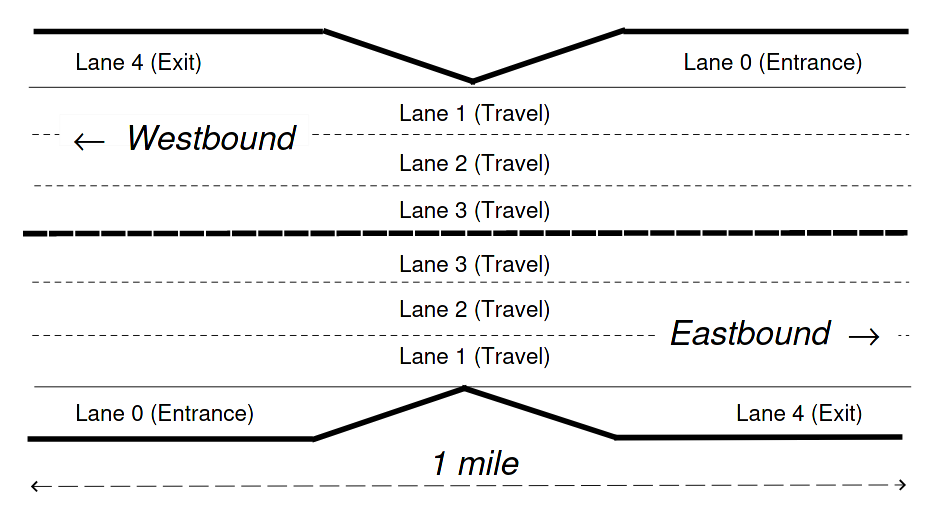
\includegraphics[scale=0.4]{lr.png}\\
        \caption{An Example Expressway Segment}
        \label{fig:lr_ex}
    \end{figure}
\end{frame}


\begin{frame}[fragile]{Queries}
    The query to execute is $SegToll$, but in order to calculate it, we need to calculate various other relations first.
    \begin{lstlisting}[language=SQL, caption= CurCarSeg linear road query]
        SELECT car_id, exp_way, dir, seg
        FROM CarSegStr [PARTITION BY car_id ROWS 1], CurActiveCars
        WHERE CarSegStr.car_id = CurActiveCars.car_id;
    \end{lstlisting}
\end{frame}

\begin{frame}[fragile]{Queries}    
    \begin{lstlisting}[language=SQL, caption= SEGAVGSPEED linear road query]
        SELECT exp_way, dir, seg, AVG(speed) as speed,
        FROM CarSegStr [RANGE 5 MINUTES]
        GROUP BY exp_way, dir, seg;
    \end{lstlisting}
\end{frame}

\begin{frame}[fragile]{Queries}
    \begin{lstlisting}[language=SQL, caption= SEGVOL linear road query]
        SELECT exp_way, dir, seg, COUNT(*) as volume
        FROM CurCarSeg
        GROUP BY exp_way, dir, seg;
    \end{lstlisting}
\end{frame}

\begin{frame}[fragile]{Queries}
    \begin{lstlisting}[language=SQL, caption= SEGTOLL linear road query]
        SELECT S.exp_way, S.dir, S.seg, basetoll*(V.volume-150)*(V.volume-150)
        FROM SegAvgSpeed as S, SegVol as V
        WHERE S.exp_way = V.exp_way and S.dir = V.dir and S.seg = V.seg
              and S.speed <= 40;
    \end{lstlisting}
\end{frame}

\begin{frame}{Implementation}
a
\end{frame}

\begin{frame}{Justification}
The things considered while determining the neural network to use for training the DQN are :-
    \begin{itemize}[<+->]
        \item To achieve a value as close as possible to the global minima for the optimization function (Adam optimzer)
        \item The time required to predict the optimal move should not exceed the time saved by using it.
        \item The time and resources required for training should not exceed the capacity of the system while it is running the query processing in the background. 
    \end{itemize}
\end{frame}

\begin{frame}{Justification}
    What we found was:-
    \begin{itemize}[<+->]
        \item Adding additional layers improves the prediction of the optimal moves but not by significant margin.
        \item Adding additional layers resulted in the time spent predicting the answer overshadowing the time saved by executing the optimal move.
    \end{itemize}
But note, these $2$ are only query and data specific findings.
\end{frame}

